% Description: 	Template for U-SPACE documentation
% Author:		Morten Olsen

% HOW TO USE THIS TEMPLATE?
%
% 1. Go to line 78 in this document and fill in the relevant information
%
% 2. Open and edit the following files: 
%		- introduction.tex
%		- requirements.tex
%		- preliminary_design.tex
%		- text_verification.tex
%		- resources_schedule.tex
%
% 3. Compile the report from this file (TEMPLATE.tex), using the following sequence:
%		a. PDFLaTex
%		b. BibTex
%		c. PDFLaTex
%		d. PDFLaTex
% 
% 4. Rename the output pdf-file, according to the document reference number (line 78 in this file)
%
% 5. Enjoy the outcome! :-)
%
% If you experience problems, try to search on Google or contact Morten Olsen
%
\documentclass[a4paper,11pt,titlepage]{article}
\usepackage[english]{babel}
\usepackage[margin=3cm]{geometry}
\usepackage[T1]{fontenc}
\usepackage[utf8]{inputenc}
\usepackage{lmodern}
\usepackage[sorting=none]{biblatex}
\usepackage{graphicx}
\usepackage{fancyhdr}
\usepackage[textfont={small,it},labelfont=bf,labelsep=endash]{caption}
\usepackage[table]{xcolor}
\usepackage{verbatim}
\usepackage[toc,page]{appendix}
\usepackage{amsmath}
\usepackage{multicol}	% allow multi column environemnt
\usepackage{float} % forced position of figures/tables etc.
%\usepackage{mathtools}
%\usepackage[framed,numbered]{mcode}
\usepackage{acronym}
\usepackage{rotating}
\usepackage{titling}
\usepackage{bibcheck}
%\usepackage{pdfpages}
%\usepackage[pdfpagemode=FullScreen,pdfstartview=FitH,pdfborder={0 0 0},pdftitle={My report},bookmarks,pdfauthor={Morten Olsen}]{hyperref}
\usepackage{memhfixc}
%\usepackage{maplestd2e}

\graphicspath{{./figures/}}	% look for graphic files in the "figures" subfolder

\definecolor{tableshade}{HTML}{E8E8E8}
\linespread{1.3}

% define the page headers and footers
\fancyhead{}
\fancyhead[RE,RO]{\parbox[b]{10cm}{\raggedleft U-SPACE\\ \today}}
\fancyhead[LE,LO]{\parbox[b]{10cm}{\docreference \\ \title }}
\renewcommand{\headrulewidth}{0.4pt}
\fancyhfoffset{1cm}
\addtolength{\headheight}{1cm}
\fancyfoot{}
\fancyfoot[C]{\thepage}
\renewcommand{\footrulewidth}{0.4pt}

\bibliography{references} % include .bib file for citations


% PLEASE FILL IN THE RELEVANT INFORMATION BELOW:
%
\def\authors{
Zhou \textsc{Hao}\\
Dries \textsc{Agten}\\
Morten \textsc{Olsen}
}
\def\docversion{DRAFT}					% Possible versions are: DRAFT, REVIEW or RELEASED
\def\docreference{USPACE-PDR-<subsystem name>-00}	% -00 = DRAFT,  -A1 = 1st release,  -A2 = 1st release with minor updates, -B1, = 2nd release
\def\title{Preliminary Design Report}
\def\subtitle{<subsystem name>}



\begin{document}

\begin{titlepage}

\begin{center}


\includegraphics[width=0.6\textwidth]{figures/logo.pdf}\\[0.75cm] 

\textsc{\large Unmanned Solar Powered Airship Concept Evaluation}\\[1cm]

\line(1,0){415}\\[1mm]
\vspace{-1.0em}
\Huge \bfseries{\title}\\[2mm] 
%\
\vspace{-1.0em}
\line(1,0){415}\\[1cm]

\begin{large}
\begin{tabular}{ll}
Document Reference No.: & \docreference\\[5mm]
Document Status: & \docversion \\[1.5cm]
\end{tabular}
\end{large}

\begin{minipage}[t]{0.49\textwidth}
\begin{flushleft} \large
\emph{Authors}\\
\vspace{-1.2em}
\line(1,0){125}\\
\footnotesize{\authors}
\end{flushleft}
\end{minipage}
\begin{minipage}[t]{0.49\textwidth}
\begin{flushright} \large
\emph{Supervisors}\\
\vspace{-1.2em}
\line(1,0){125}\\
Kjell \textsc{Lundin}\\
Alf \textsc{Wikstr\"{o}m}
\end{flushright}
\end{minipage}

\vspace{1cm}

\begin{minipage}[t]{0.49\textwidth}
\begin{flushleft} \large
\emph{Project Manager}\\
\vspace{-1.2em}
\line(1,0){125}\\
Dries \textsc{Agten}
\end{flushleft}
\end{minipage}
\begin{minipage}[t]{0.49\textwidth}
\begin{flushright} \large
\emph{Quality Manager}\\
\vspace{-1.2em}
\line(1,0){125}\\
Morten \textsc{Olsen}\\[1cm]
\end{flushright}
\end{minipage}

\vfill

\begin{large}
\today \\
Lule\r{a} University of Technology \\
Rymdcampus, Kiruna, Sweden\\
\end{large}

\end{center}

\end{titlepage}

\pagestyle{plain}
\pagenumbering{roman}

\thispagestyle{plain}
\chapter*{Acronyms}
\markboth{Acronyms}{Acronyms}
\addcontentsline{toc}{chapter}{\protect\numberline{}Acronyms}

\begin{multicols}{2}
\begin{acronym}
\acro{ADCS}{Attitude determination and control}
\acro{ADC}{Analog to Digital converter}
\acro{ADS}{Attitude Determination System}
\acro{BCR}{Battery Charge Regulator}
%\acro{BJT}{Bipolar Junction Transistor}
%\acro{CC}{Constant Current}
\acro{CDR}{Critical Design Review}
%\acro{CM}{Current Mode}
\acro{COTS}{Commercial Off-The-Shelf}
\acro{CPU}{Central Processing Unit}
\acro{CRC}{Cyclic Redundancy Check}
%\acro{DCM}{Discontinuous Conduction Mode}
\acro{DM}{Development Model}
\acro{DSP}{Digital Signal Processor}
\acro{ECSS}{European Cooperation for Space Standardization}
\acro{EGSE}{Electrical Ground Support Equipment}
\acro{EKF}{Extended Kalman Filter}
\acro{EMC}{Electromagnetic Compatibility}
\acro{EMI}{Electromagnetic Interference}
\acro{EPS}{Electrical Power System}
\acro{ESC}{Electronic Speed Control}
%\acro{ESR}{Equivalent Series Resistor}
\acro{ETSI}{European Telecommunications Standards Institute}
\acro{FM}{Flight Model}
%\acro{FRR}{Flight Readiness Review}
\acro{GPS}{Global Positioning System}
\acro{$I^2C$}{Inter-Integrated Circuit}
\acro{IC}{Integrated Circuit}
%\acro{IDC}{Insulation Displacment Connector}
\acro{IRF}{Swedish Institute of Space Physics}
\acro{ISE}{Integrated software environment}
\acro{ITPU}{Imaging and Tracking Payload Unit}
\acro{ITU}{International Telecommunication Union}
\acro{LDO}{Low-dropout}
\acro{LiPo}{Lithium-Polymer}
\acro{LTU}{Lule\r{a} University of Technology}
\acro{MCC}{Motor Control and Communication}
\acro{MCU}{Micro-Controller Unit}
%\acro{MEA}{Main Error Amplifier}
\acro{MGSE}{Mechanical Ground Support Equipment}
%\acro{MOSFET}{Metal-Oxide-Semiconductor Field-Effect Transistor}
%\acro{MPP}{Maximum Power Point}
\acro{MPPT}{Maximum Power Point Tracking}
%\acro{MPPTU}{Maximum Power Point Tracking Unit}
\acro{MSE}{Mechanical Structure and Envelope}
%\acro{NTC}{Negative Temperature Coefficient}
\acro{OBDH}{Onboard Data Handling}
%\acro{OpAmp}{Operational Amplifier}
\acro{OSI}{Open Systems Interconnection}
\acro{PCB}{Printed Circuit Board}
\acro{PDR}{Preliminary Design Review}
%\acro{SA}{Solar Array}
%\acro{PSA}{Pressure Sensitive Adhesive}
%\acro{PTC}{Positive Temperature Coefficient}
\acro{PWM}{Pulse Width Modulation}
%\acro{RHPZ}{Right Half Plane Zero}
\acro{RMP}{Rounds Per Minute}
\acro{SAR}{Solar Array Regulator}
\acro{SD}{Secure Digital}
\acro{SMD}{Surface-Mount Device}
\acro{SoC}{System on Chip}
\acro{SPA}{Solar Powered Airship}
\acro{SSC}{Swedish Space Corporation}
\acro{TBD}{To Be Decided}
\acro{U-SPACE}{Unmanned Solar Powered Airship Concept Evaluation}
\acro{UART}{Universal Asynchronous Receiver/Transmitter}
%\acro{UAS}{Unmanned Aircraft System}
%\acro{UAV}{Unmanned Aerial Vehicle}
\acro{USB}{Universal Serial Bus}
\acro{UVLO}{Under-Voltage Lock-Out}
\acro{TTC}{Telemetry, Tracking and command}
\acro{ISM}{Industrial, Scientific and Medical}
\acro{RF}{Radio Frequency}
\acro{TC}{Telecommand}
\acro{TM}{Telemetry}
\acro{URL}{Uniform Resource Locator}
\end{acronym}
\end{multicols}

\markboth{List of Figures}{List of Figures}
\addcontentsline{toc}{section}{\protect\numberline{}List of Figures}
\listoffigures
\newpage

\markboth{List of Tables}{List of Tables}
\addcontentsline{toc}{section}{\protect\numberline{}List of Tables}
\listoftables
\newpage

\tableofcontents
\newpage
\acresetall	%reset acronyms which is otherwise used in list of figures or tables
\clearpage %reset page numbers
\pagenumbering{arabic}
\pagestyle{fancy}

\chapter{Basic LaTex Commands}
This section provides some basic useful LaTex commands. For further reference, search on Google where you will find plenty of useful LaTex blogs. \textbf{Remove this chapter later on...}

\section{Figures}

This is a figure example:

\begin{figure}[H] % the "H" specifies to place the figure exactly here in the document - If left out, LaTex will sometimes place figures a bit awkwardly.
\centering

\includegraphics[scale=1]{Drawing1} % it is recommended to use pdf or another vector graphic file for optimal quality
\caption{This is a figure caption}
\label{fig:figure1_label}
\end{figure}

You can also place figures side-by-side. An easy way is to use a "minipage" environment:

\begin{minipage}[b]{0.45\linewidth}  % "b" means that the bottom-line of the "minipages" will be aligned
\begin{figure}[H]
\centering

\includegraphics[width=0.9\textwidth]{Drawing1}
\caption{This is a figure caption}
\label{fig:figure2_label}
\end{figure}
\end{minipage}
\hspace{2mm} % include some horizontal space between the two figures
\begin{minipage}[b]{0.45\linewidth}
\begin{figure}[H]
\centering

\includegraphics[width=0.7\textwidth]{Drawing1}
\caption{This is a figure caption}
\label{fig:figure3_label}
\end{figure}
\end{minipage}

An alternative is to use the "subfigure" command inside the "figure" environment. You need the
\begin{verbatim}
\usepackage[center]{subfigure}
\end{verbatim}
command in your preamble. With this command, the figures will be labelled a, b, c etc.

\begin{figure}[htbp!]
\centering
\subfigure [Caption for subfigure 1]{\label{fig:figure4_label}
\includegraphics[width=0.49\textwidth]{Drawing1}}
\subfigure [Caption for subfigure 2]{\label{fig:figure5_label}
\includegraphics[width=0.49\textwidth]{Drawing1}}
\caption{General caption} 
\label{fig:figure4_5_label}
\end{figure}

\section{Tables}

This is an example of a table:

\begin{table}[H]
\centering
\caption{This is a table caption}
\label{tab:table1_label}
\begin{tabular}{|l|l|l|} % "|" means a border, "l" means left-aligned text in cells.
\hline % adds a horizontal border
\textbf{Header 1} & \textbf{Header 2} & \textbf{Header 3}\\ %use "&" to separate cells and remember a "\\" linebreak in the end
\hline 
Some text & Some text & Some text\\
Some more text & Some more text & Some more text\\
\hline
\end{tabular}
\end{table}

You can also do a table with multi-line cells:

\begin{table}[H]
\centering
\caption{This is a table caption}
\label{tab:table2_label}
\begin{tabular}{|p{0.4\textwidth}p{0.3\textwidth}p{0.2\textwidth}|}
\hline
\textbf{Header 1} &  \textbf{Header 2} & \textbf{Header 3}\\ 
\hline
Some long text that does not fit in a single-line table cell & Some text & Some text \\
Some more text & Another very long text that does not fit in a single-line table cell & Some more text\\
\hline
\end{tabular}
\rowcolors{3}{tableshade}{white}	% adds alternating background color of the table rows
\end{table}

\section{Equations}

You can do simple in-line equations by using the "\$" symbols around the equation: $2+2=4$. Remember always to use a the math- or equation environment when using variables like $+$, $=$, $x^{2}$, $f_{2}$ etc.

To write a numbered equation on its own line, use the "equation" environment: 

\begin{equation}
\label{eq:equation1_label}
T(s)=\frac{G(s)H(s)}{1+G(s)H(s)}
\end{equation}

You can also do multi-line equation by using the "split" - environment:

\begin{equation}
\begin{split}
\label{eq:equation2_label}
2x+4y&=6\\	%use "&" to align the equations over the same point
4y&=6-2x\\
y&=1.5-0.5x\\
\end{split}
\end{equation}

\section{Citations, References and Acronyms}

This is a citation\cite{CitationReference1}.

This is a citation referring to a specific page in the cited work\cite[28]{CitationReference1}. 
\\
You can also do multiple citations\cite{CitationReference1,CitationReference2}.

This is a cross-reference to a figure/section/table/equation etc. in the latex document: see Figure \ref{fig:figure1_label}.
\\
Use acronyms consistently to provide an easy-reading text: The \ac{U-SPACE} project rocks!
\newpage
\section{Introduction}
\label{sec:introduction}

The \ac{EPS} provides power to motors, the on-board computer, communication system and payloads. Power is mainly supplied from solar cells but can also be supplied from a battery, when solar power is not available or insufficient. 

\subsection{Changes from PDR to CDR}
\label{sec:changes_pdr_to_cdr}
%
Table \ref{tab:pdr_to_cdr} lists major design changes from the \ac{EPS} \ac{PDR} report.

\begin{table}[H]
\centering
\caption{U-SPACE \ac{EPS} design changes from PDR to CDR}
\label{tab:pdr_to_cdr}
\begin{tabular}{p{0.25\textwidth}p{0.2\textwidth}p{0.45\textwidth}}
\hline
\textbf{Area of change} & \textbf{Changed parameter } & \textbf{Argumentation for change}\\
\hline
Total power budget & Increased to $>40\,W$ & Airship total mass and size are increased thus requiring much more power for the motors\\
Solar cells & New part & Old solar cell was much heavier than listed in manufacturer datasheet due to a glass cover\\
Total system cost & Increased to $>12000\,SEK$ & Increased power and new light-weight solar cells are more expensive\\
Solar cell mounting & New part & New solar cell is flexible instead of rigid and can be mounted with \ac{PSA}\\
\hline
\end{tabular}
\end{table} 
\chapter{Goals and Constraints}
\label{chap:goals_constraints}

\section{Project Goals}
\label{sec:goals}
%What function(s) does the subsystem have to fulfill?

The principal goal of the \ac{U-SPACE} project is to try and bridge the gap between a student-driven engineering project and the concept of an unmanned \ac{SPA}. As very few examples of this type of design exist \cite{website:solr}, much is to be gained from this project. Due to the many constraints that have to been taken into account (see section \ref{sec:constraints}), the goal is necessarily modest. The goal of this project is thus designing, building and testing a small-scale \ac{SPA} for low altitude flight, including support for a scientific payload. The basic targets are listed below:

\begin{itemize}
\item Design of a small unmanned \ac{SPA} capable of forward propulsion, powered by solar cells and including a scientific payload
\item Construction of such an \ac{SPA} with minimal cost
\item Flight test of this \ac{SPA} at low altitude
\end{itemize}

\section{Project Constraints}
\label{sec:constraints}
%What technical requirements constrain the subsystem design? - e.g. mass, power, strength, stability etc.

The design, construction and test of a small unmanned \ac{SPA} is susceptible to many constraints, all of which have to be identified, examined and finally dealt with. These constraints take many forms, but may be divided into four categories: functionality, resources, environment and law.

\subsection{Functionality}

The \ac{U-SPACE} project, being a proof of concept, consists of designing, building and testing a small version of a \ac{SPA} with a limited scientific payload. Therefore reasonable limits have to be taken into account for some technical parameters. These parameters and their limits are listed below in table \ref{tab:functionality}.

\begin{table}[H]
\centering
\caption{Functional parameters and limits}
\label{tab:functionality}
\begin{tabular}{c c c}
\hline
\textbf{Parameter} & \textbf{Lower limit} & \textbf{Upper limit}\\ \hline
Total mass & / & 4.5 kg\\
Flight altitude & 2 m & 100 m\\
Electrical power & / & 40 W\\
Forward velocity & / & 1 m/s\\
Radius & 10 m & /\\
\hline
\end{tabular}
\end{table}

\subsection{Resources}

Since the \ac{U-SPACE} project is a student project supported by \ac{LTU} and \ac{IRF}, the available resources are limited. This imposes stringent constraints on all phases of the project. The main resources can be identified as the three elements of the project management triangle, shown in figure \ref{fig:project_triangle}.

\begin{figure}[htbp!]
\centering
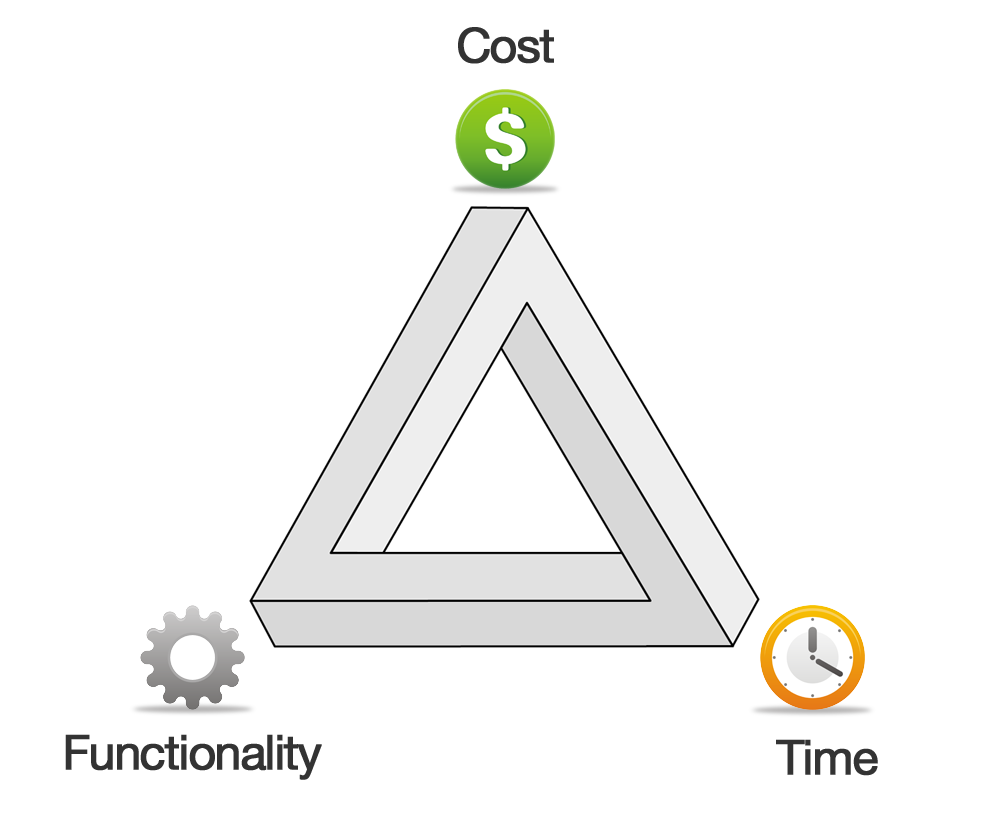
\includegraphics[scale=0.2]{figures/project_triangle.png}
\caption[Project management triangle]{Project management triangle \cite{website:claromentis}.}
\label{fig:project_triangle}
\end{figure}

\noindent
The cost of this student project is limited by its approved budget, a sum between 10,000 and 12,500 SEK, provided by \ac{LTU}. More funding can be applied for if required, but the budget nevertheless remains limited. This constraint implies a careful selection of components and the use of innovative engineering solutions throughout the entire project. 
\\
\\
The time available for this project is also constrained, being a student project that has to be realized in concurrence with other academic duties. The estimated time frame is therefore between 2 and 6 months for a first prototype capable of test flight.
\\
\\
The final resource is related to the previously mentioned functionality. With a limited number of team members that have limited expertise in the field of airships, the project has to be technically balanced, taking into account the capabilities of the members of the team.

\subsection{Environment}

The \ac{SPA} that will be developed during the \ac{U-SPACE} project finally has to be tested outdoors. Since the \ac{U-SPACE} project is being executed in the city of Kiruna during the spring, summer and early autumn, it is important to take the environmental conditions during this period of the year into account.  Some of the these conditions are listed below in table \ref{tab:environment}, using data for the month of May \cite{website:weatherspark} as a representation of the entire project period.

\begin{table}[H]
\centering
\caption{Environmental conditions}
\label{tab:environment}
\begin{tabular}{p{0.35\textwidth} p{0.15\textwidth} p{0.15\textwidth} p{0.35\textwidth}}
\hline
\textbf{Parameter} & \textbf{Lower boundary} & \textbf{Upper boundary} & \textbf{Remarks}\\ \hline
Temperature & -2 $^\circ$C & 11 $^\circ$C & Average values\\
Wind speed & 1 m/s & 6 m/s & Usually from the south west\\
Probability of precipitation & 61 \% & 61 \% & Average value\\
Hours of sunshine & 17:38 h & 22:45 h & Daily values\\
Cloud cover & 83 \% & 83 \% & Median value\\
Solar incidence angle at noon & 46 $^\circ$ & 46 $^\circ$ & Refer to document USPACE-PDR-PWR-A1\\
\hline
\end{tabular}
\end{table}

\subsection{Law}

The final constraints that have to be taken into account are possible legal issues that may arise during the construction and testing of the \ac{SPA}. A first legal constraint is the compliance to the \ac{ITU} Radio Regulations \cite{book:freqalloc} when using wireless connections. Secondly, when flying the \ac{SPA}, the Swedish Transport Agency's regulations on \ac{UAS} \cite{regulations:uas2009} might have to be taken into account. As these application of these regulations depends on the final mass and size of the prototype airship, this constraint can only be investigated when a prototype is constructed.

\section{Expected Functionality}
%What are the expected performances of the subsystem, as related to the requirements above? (maybe including some margins)

Based on the project goals set forth in section \ref{sec:goals} and taking into account the constraints discussed in the previous section, a realistic prediction of the functionality of the final product of the \ac{U-SPACE} project can be made. The expected functionality of the small-scale \ac{SPA} are summarized in table \ref{tab:expected}.

\begin{table}[H]
\centering
\caption{Expected functionality}
\label{tab:expected}
\begin{tabular}{c c c c}
\hline
\textbf{Parameter} & \textbf{Value} & \textbf{Remarks}\\ \hline
Autonomy & 2 h & At peak power\\
Flight altitude & 2-20 m & /\\
Forward velocity & 0.5-1 m/s & /\\
Flight conditions & Daytime & Sunny and calm weather\\
\hline
\end{tabular}
\end{table}

\noindent
The other functional constraints presented in section \ref{sec:constraints} will be discussed in subsequent chapters. In the future, this functionality might be expanded with features like autonomous attitude control and altitude control during flight.

\section{Fault Tolerance Design and Safety Concept}

Since the goal of the \ac{U-SPACE} project is to design, build and test a prototype of a small-scale \ac{SPA} the focus of this project is not on a fault-tolerant design of the airship, but rather on a performant design that meets the project goals. Nevertheless some safety features are included in the design, construction and flight test of the airship. These features will be discussed in the chapters dedicated to the different subsystems and in chapter \ref{chap:ground_support}.

\section{Materials}

With the limited time and funding inherent to this student-driven project great care needs to taken with regards to the selection and processing of the materials. The materials need to be as performant as possible for their specific function while at the same time their cost should be as low as possible. In general all materials should also be as light as possible. The specific material requirements for each subsystem are discussed in the subsequent chapters.
\\
\\
With regards to the processing of the materials, low cost is again the main discriminator to select an appropriate technique. Therefore the simplest techniques are preferred during the construction of the airship, with as less mechanical work as possible. A certain amount of experience with such techniques is present in the team, allowing short construction times and limited delays.
\section{Preliminary Design}
\label{sec:preliminary_design}
%\subsection{Preliminary Design Explanation}
%Explain the preliminary design including block diagrams, schematics, drawings, etc.
%Modular design - easy for scaling
%Output voltage level trade analysis
%Analysis of "orbit"
%Component ratings considerations
%Possible up-scaling of system - larger power, modular design, higher voltage?
%Load profile/switching: motors, communication, payload(s), OBDH?, sensors, regulators?,
%Decide on sufficient design margins?
%EMI/EMC/ESD for scientific payloads and safety
%Look into previously flown solar powered airships
%Scalability to fly in high-altitude "orbits" i.e. temperatures, reliability, ionization?, 
%Possibility to cover "wings" with solar cells - trade study of benefit!
%Payload short-circuit
%
\subsection{Solar Array Design}
%Bypass diodes on SA to mitegate shadowing problems
%Cross-strapping of solar cells?
%\subsubsection*{Solar Array Shading}
%Bypass diodes can be used to partly mitigate this issue as well as using \ac{MPPT}. Otherwise it could be necessary to ensure that the airship structure cannot cast shadows on the panels and that the airship only fly above or away from landscape objects.
%SA isolation diodes
%
Section \ref{subsec:environmental_requirements} discussed the importance of the sun incidence angle on the solar panels. It is first considered having the solar array divided into two identical panels on each side of the airship. Considering that the sun incidence is directly falling on one of the sides of the airship, the "back-side" solar panel on the airship may still produce power, if the incidence angle is not too large. Considering the Kelly cosine function from figure \ref{fig:KellyCosine}, the maximum total output current (power), from each solar panel, is around $71\%$, when both solar panels are at $90^{\circ}$ angles (completely flat on top of the airship). In practical, having complete flat panels on top of the airship is hard to realize and a compromise must be made. Hence, the panels should be angled as small as possible, to maximize the total power output.

The same issue goes for the changing sun incidence angle due to the flight attitude around the vertical axis. Again, ideally the solar panels should be flat on the top of the airship. In practical, it is more realistic to place four identical solar panels on top of the airship, with as small an angle as possible with respect to vertical. The proposed layout of the four solar panels is illustrated in figure \ref{fig:solar_panels_mounting}.
%
\begin{figure}[H]
\centering
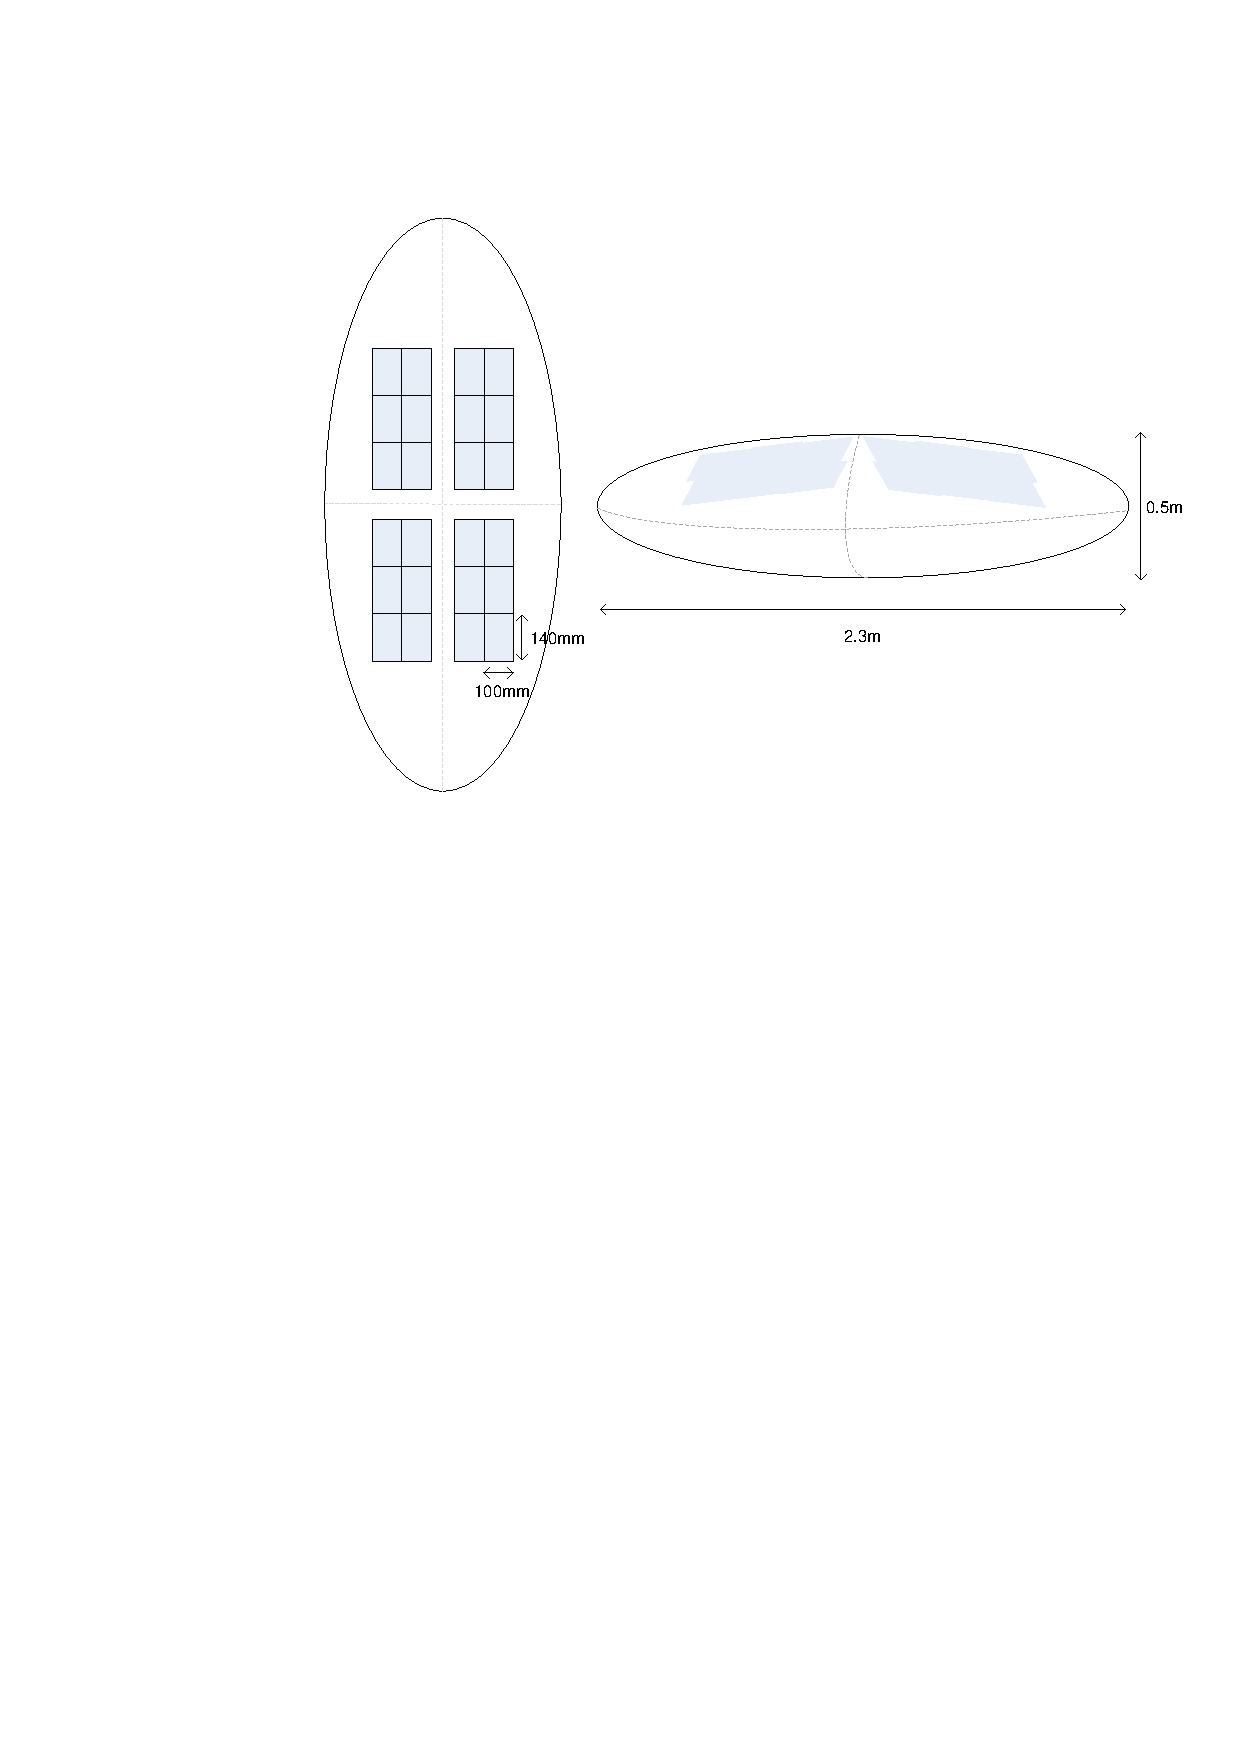
\includegraphics[scale=0.8]{figures/fig_PDR_Solar_Panels_Mounting}
\caption{Mounting of the solar panels}
\label{fig:solar_panels_mounting}
\end{figure}
%
The proposed solar cell, \cite{MC_Solar_Cell}, has the following current and voltages at the \ac{MPP}:
%
\begin{equation}
\begin{split}
V_{cell,MPP}&=3.85\,V\\
I_{cell,MPP}&=210\,mA
\end{split}
\end{equation}
%
Each of the four panels will consist of six solar cells giving a maximum power output of:
%
\begin{equation}
\begin{split}
P_{panel,MPP}&=6\cdot V_{cell,MPP}\cdot I_{cell,MPP}\\
P_{panel,MPP}&=4.85\,W
\end{split}
\end{equation}
%
It is considered having two series-connected cells and three in parallel, thus having an output voltage of: 
%
\begin{equation}
V_{panel,out}=7.7\,V
\end{equation}
%A future upgrade of the project, could including a simple solar array drive mechanism for each solar panel. This could increase the solar arrays output and make the design more flexible for flying in varying solar incidence angles, i.e. different seasons, latitudes or time of day. However, this approach is more complicated and not applicable for the U-SPACE project.
%

%
\subsection{Regulator Design}
%Which design concepts are considered? - What are the advantages/disadvantages for each concept?
%Decide on MPPT algorithm (using analog circuits?)
%DC-DC regulator topology (Buck, Boost, Buck-Boost etc.)
%
%
An important trade-off analysis is the selection of the \ac{SAR}. Table \ref{tab:TradeOff} shows the comparison between three possible regulators. These three are shortly described below:
%
\subsubsection*{Zener Diode Regulator}
The most simple design is to use a Zener-diode regulator, as shown in figure \ref{fig:zenerdiode_regulator}. The circuit comprises a Zener-diode with a reverse break-down voltage equal to the desired output voltage. Excessive current from the solar arrays runs through the Zener-diode, thus keeping the load current and output voltage constant. The resistor is included to limit the current drawn by the Zener-diode to protect it from over-currents. Since a series resistor is inserted, significant  power losses are experienced and therefore this circuit is only useful in low power applications. 
%
\begin{figure}[H]
\centering
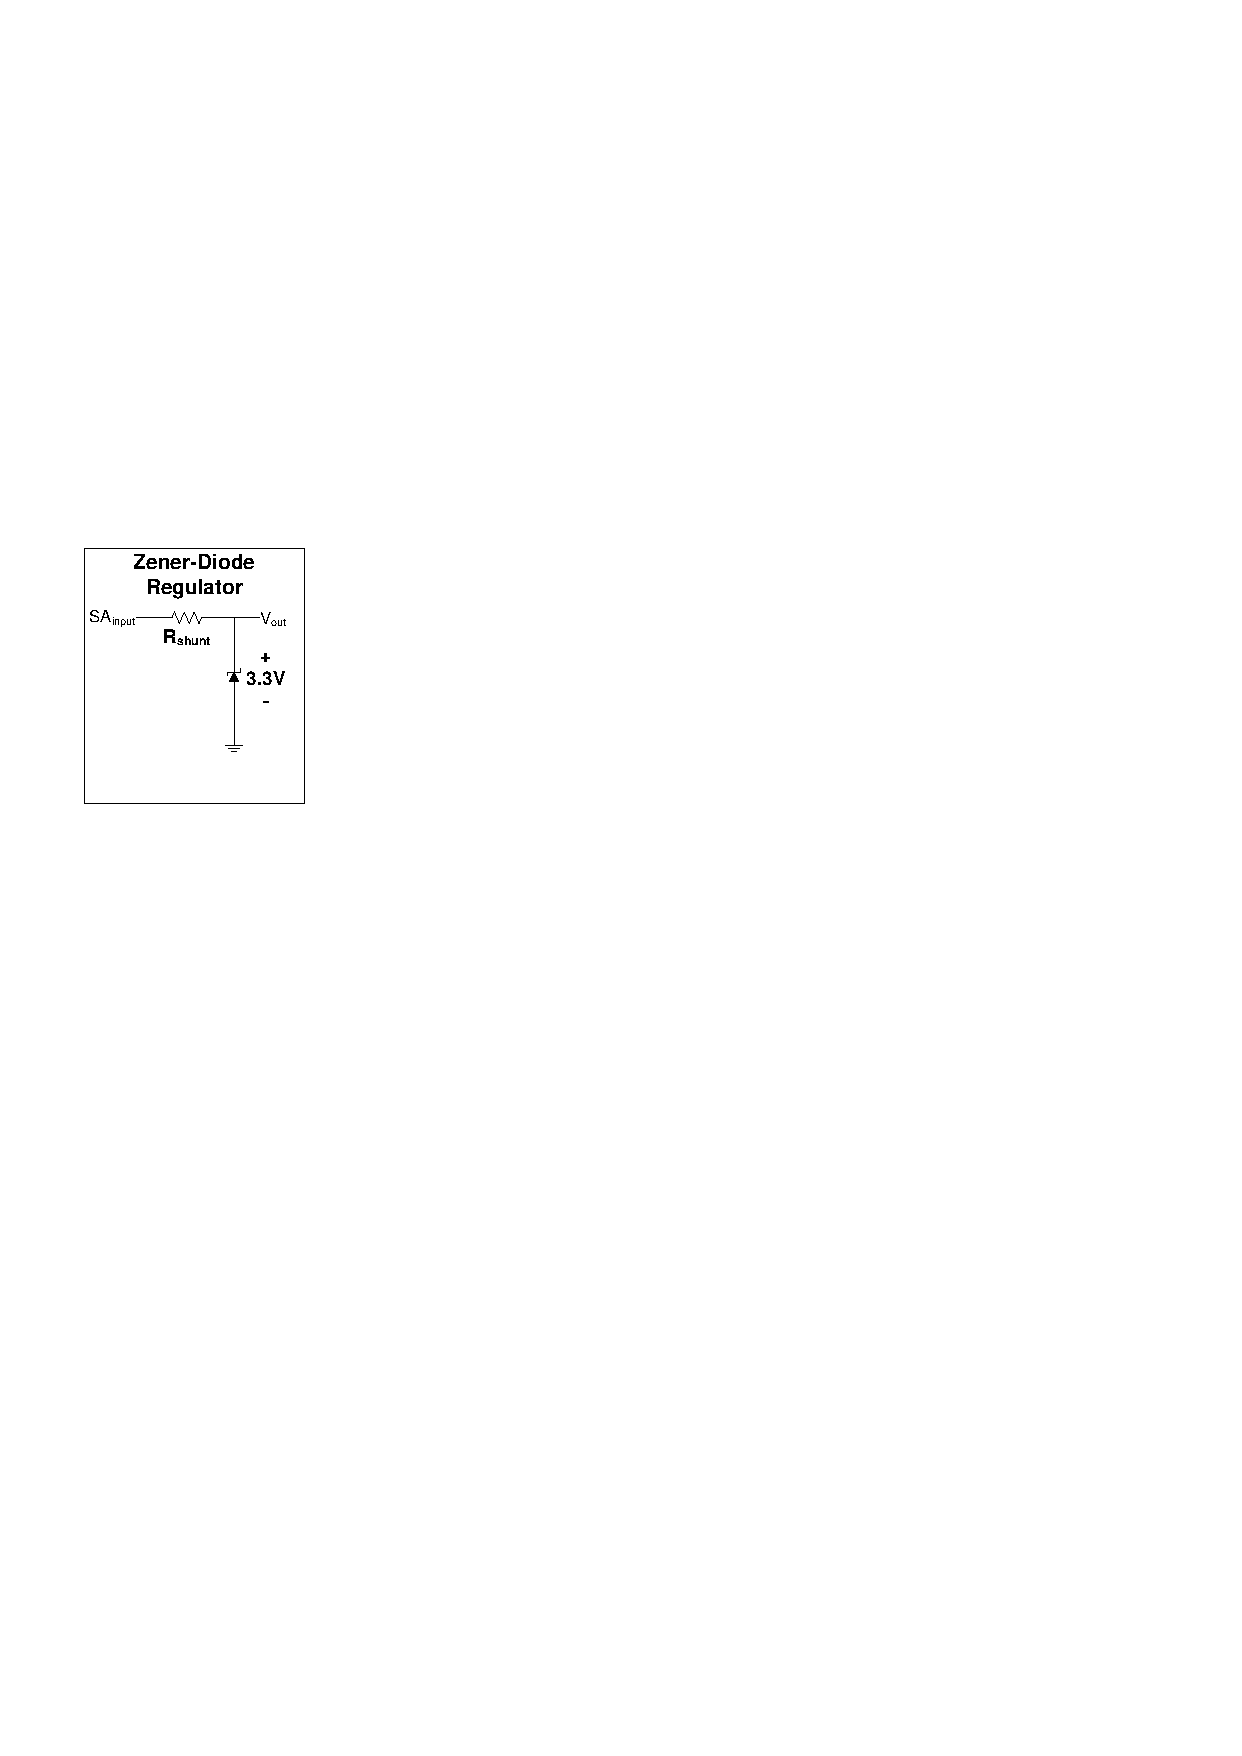
\includegraphics[scale=1]{figures/fig_PDR_Zenerdiode_Regualtor}
\caption{Simple Zener-diode regulator}
\label{fig:zenerdiode_regulator}
\end{figure}
%
%
\subsubsection*{Shunt Regulator}
The shunt regulator concept also uses a shunt resistor, but the Zener-diode is replaced by a transistor. When the transistor is closed, the solar array current is shorted to ground through the shunt resistor. A feedback line measures the output voltage, compares it to a reference voltage and generates a control signal. This signal is fed to a \ac{PWM} driver for the transistor gate. This way, the current supplied to the load can be controlled and the output voltage kept constant. The solar array will operate at the same voltage as the output voltage. By manually changing the reference voltage, the output voltage could be changed, thus adding some degree of flexibility for operating conditions of the solar array. The shunt-regulator concept is shown in figure \ref{fig:shunt_regulator}.
%
\begin{figure}[H]
\centering
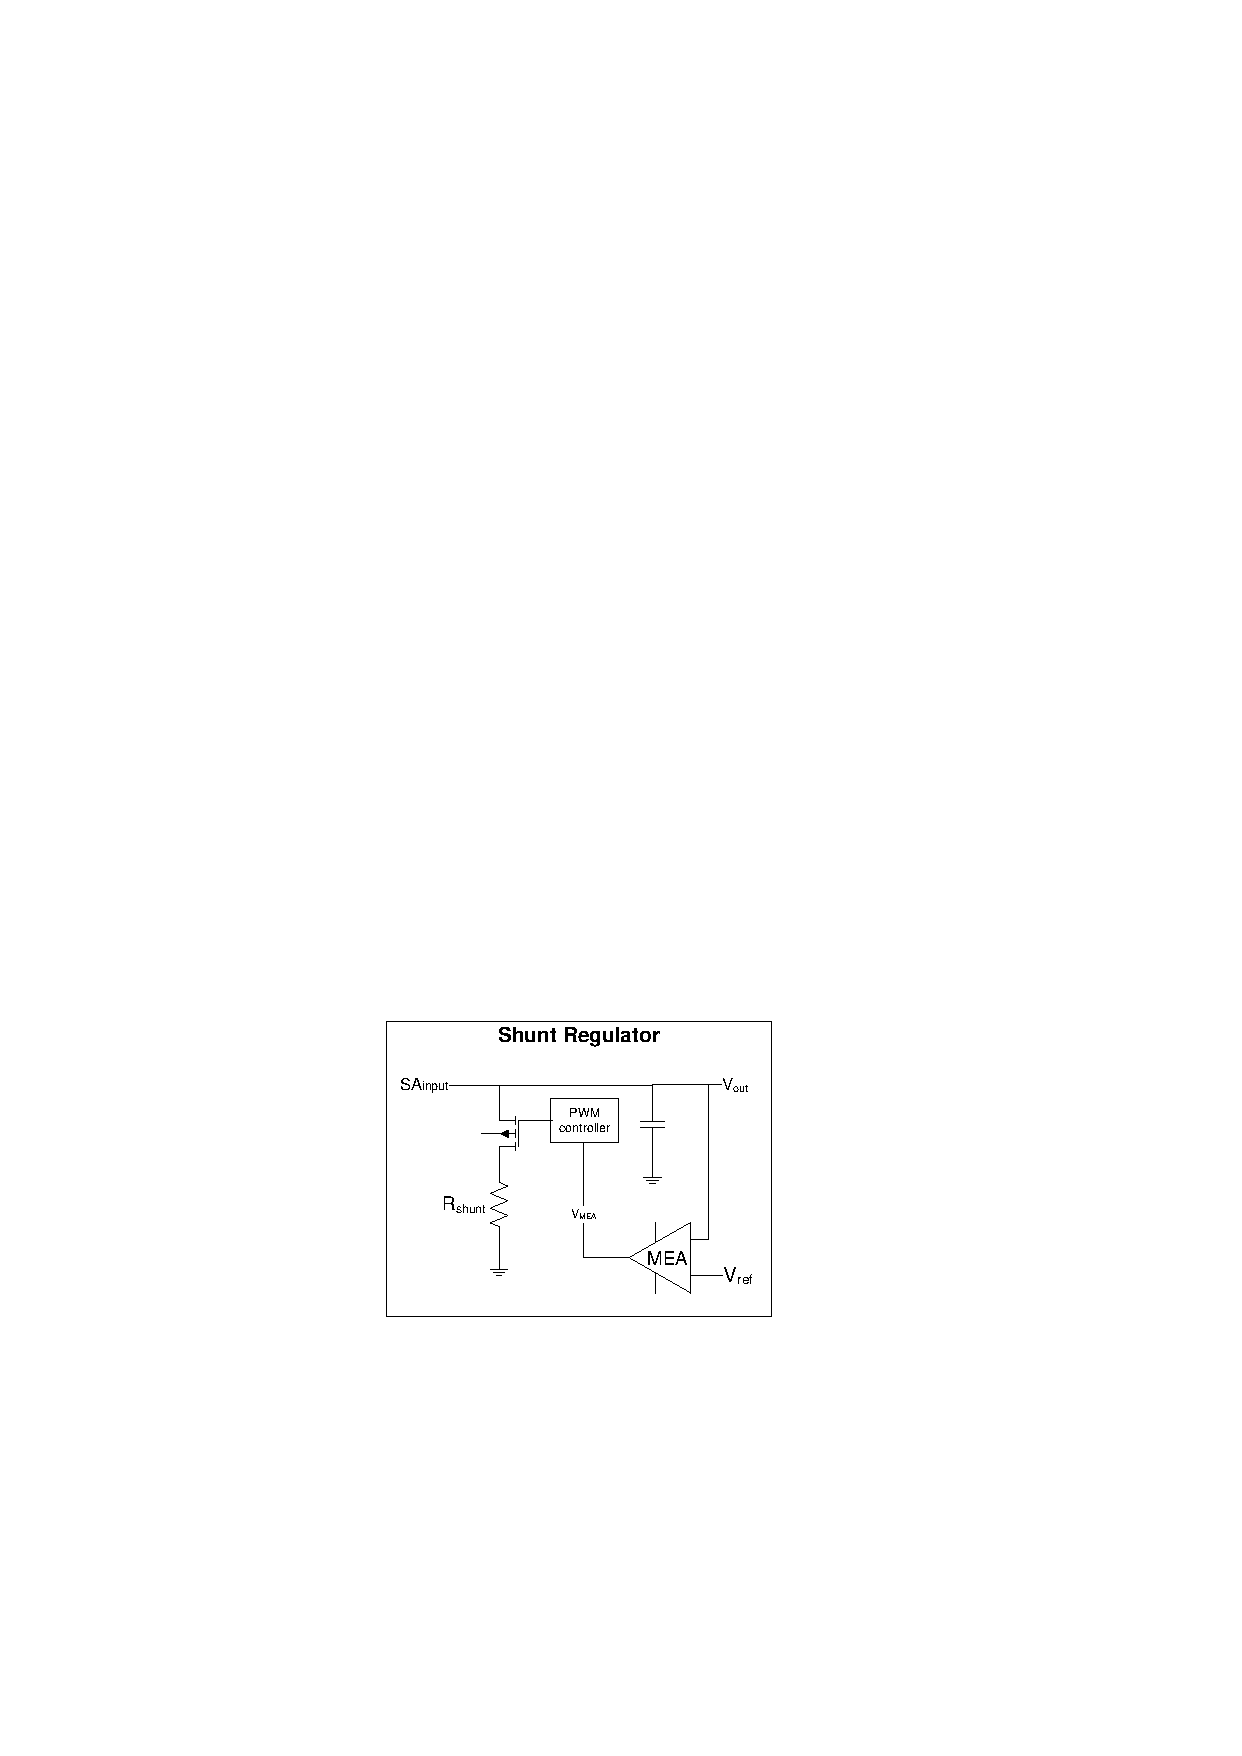
\includegraphics[scale=1]{figures/fig_PDR_Shunt_Regulator}
\caption{Shunt regulator diagram}
\label{fig:shunt_regulator}
\end{figure}
%
\subsubsection*{Maximum Power Point Tracking Regulator}
The most advanced and robust solution is to use an \ac{MPPT} regulator as shown in figure \ref{fig:MPPT_regulator}. A standard DC-DC converter topology (buck or boost) is used, comprising a transistor, free-wheel diode, inductor and output capacitor. Like in the shunt-regulator, the output voltage is measured and compared to a reference voltage, to generate a \ac{PWM} control signal, to drive the transistor. By varying the duty cycle of the \ac{PWM} signal, the input voltage (solar array operating voltage) can be controlled. Additionally an \ac{MPPT} circuit is added. The solar array current and voltage are measured and fed to the circuit which then calculates the power output of the solar array. By making small steps in the solar array operating voltage, the characteristic IV-curve of the solar array can be generated and the \ac{MPP} can be tracked, thus always operating the solar array at is optimal operating point. When using an \ac{MPPT} regulator, three operating modes will be possible:
%
\begin{itemize}
\item Battery discharge {MPPT} - when the solar array input power is insufficient to cover the load power demand, the battery is slowly discharged in order to maintain the output voltage.
\item Battery charge {MPPT} - when the solar array input is greater than the load power, the excessive power is used to recharge the battery.
\item Input power limitation - when the battery is fully charged, the regulator will operate the solar array at a non-optimal voltage, thus limiting the input power to keep the output voltage constant. The extra potential input power is dissipated as heat externally on the solar arrays.
\end{itemize}
%
\begin{figure}[H]
\centering
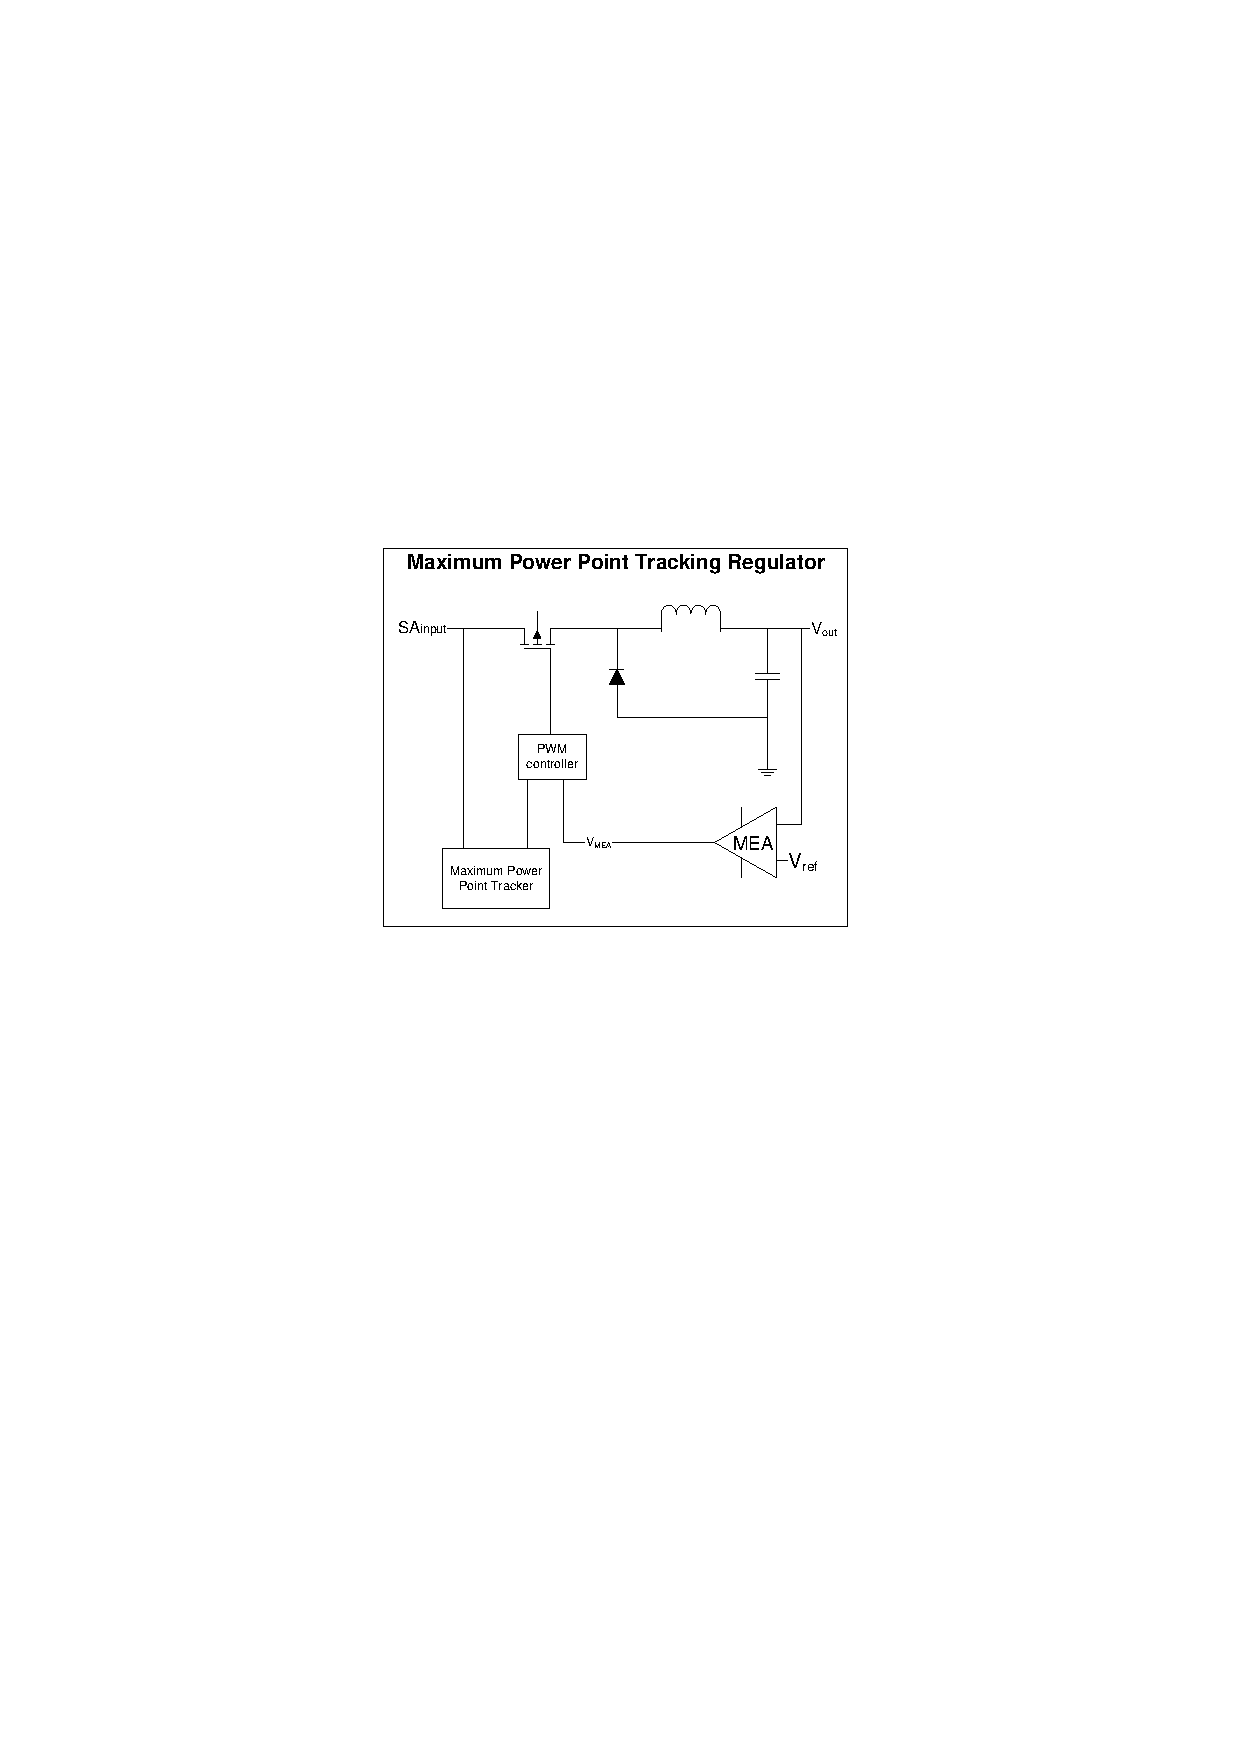
\includegraphics[scale=1]{figures/fig_PDR_MPPTdiagram}
\caption{\ac{MPPT} regulator diagram}
\label{fig:MPPT_regulator}
\end{figure}
%
%
%\begin{center}
\begin{table}[H]
\centering
\rowcolors{3}{tableshade}{white}
\caption{Trade off analysis}
\label{tab:TradeOff}
\begin{minipage}{\textwidth}
\centering
\begin{tabular}{||p{0.22\textwidth}p{0.22\textwidth}p{0.22\textwidth}p{0.22\textwidth}||}
\hline
\textbf{SA Regulator Concepts:} &  \textbf{MPPT} & \textbf{Shunt-Regulator} & \textbf{Zener-diode Regulation}\\ 
\hline
Costs & Medium(some ICs required) & Medium(some ICs required) & Low(simple components)\\
Regulator efficiency & High($90-95\%$) & Medium($70-95\%$) & Low($40-70\%$\footnote{Efficiency drops significantly at high current loads, due to the shunt resistor})\\
Size/mass & $\sim140-240 g$\footnote{up to four identical circuits are needed, one for each solar panel, hence the larger mass} & $\sim50 g$ & $\sim45 g$\\
Output voltage stability & Good & Average & Poor\\
Scalability & Very good & Average & Poor\\
Internal heat dissipation & Low & Medium & High\\
Complexity & High & Medium & Low\\
Flexible to variations(temperature, shading, degradation) & Very good & poor (only manually) & none\\
Implementation time & $\sim1-2\,months$ & $\sim3-4\,weeks$ & $< 1\,week$\\
\hline
\end{tabular}\par
\vspace{-0.75\skip\footins}
\renewcommand{\footnoterule}{}
\end{minipage}
\end{table}
%\end{center}
%
\subsection{Battery Design}
%
A trade-off analysis between different battery chemistry has been conducted and the results are listed in table \ref{tab:TradeOff_battery}. 
%
%Battery overcharge
%Battery charge limitation
%Battery short-circuit?
%Charge regulation: Bulk, Taper, Trickle-charging.
%Battery maximum charge ratio
%Battery maximum discharge ratio
%Battery maximum Depth of Charge (DOD)
%
%
\begin{center}
\begin{table}[H]
\rowcolors{3}{tableshade}{white}
\caption{Trade off analysis}
\label{tab:TradeOff_battery}
\begin{tabular}{||p{0.1\textwidth}p{0.40\textwidth}p{0.40\textwidth}||}
\hline
\textbf{Battery type} &  \textbf{Advantages} & \textbf{Disadvantages}\\ 
\hline
NiCd & ? & Has memory effect and toxic Cadmium\\
NiH2 &  More robust to over-charge/discharge & Low energy density, high self-discharge rate and the pressurized cell is more dangerous to handle\\
NiMH & No internal pressure, higher energy density and less sensitive to temperature & Cannot deliver high peak power, high self-discharge rate, sensitive to high temperatures and is damaged by over-charging\\
Li-ion & Highest energy density, high charge efficiency and supports high charge/discharge rates due to low internal impedance & Expensive, damaged by over-charging/discharging, sensitive to low temperatures and increased internal impedance at low temperatures\\
AgZn & High specific energy, stable cell voltage during dis-charge & Short life time\\
\hline
\end{tabular}
\end{table}
\end{center}
%
It is proposed to use a Panasonic PA-LN19 Li-ion battery \cite{Panasonic}. The battery has the following important specifications:
%
\begin{table}[H]
\centering
\caption{Specification of proposed battery}
\label{tab:proposed_battery}
\begin{tabular}{ll}
\hline
Battery chemistry & Li-ion\\
Battery voltage & $3.6\,V$\\
Battery capacity & $2.9\,Ah$ / $10.44\,Wh$\\
Weight & $49\,g$\\
\hline
\end{tabular}
\end{table}
%
\subsection{Argumentation for Chosen Concept(s)}
%Why is the chosen concept selected?
%
It is proposed to use the \ac{MPPT} concept, since this provides the most efficient and robust design and easy scales up to a larger system if/when required. It also mitigate design challenges occurring due to varying environment conditions, i.e. temperature, weather etc.

For the battery, Li-ion technology offers the most compact design ensuring low weight and relative high energy capacity.

The complete \ac{EPS} diagram is shown in figure \ref{fig:EPSdiagram}. For providing the $5\,V$ regulated voltage to the payloads, \ac{COTS} DC-DC regulator(s) are used. The battery charging/discharging is controlled by the \ac{SAR}.
%
\begin{figure}[H]
\centering
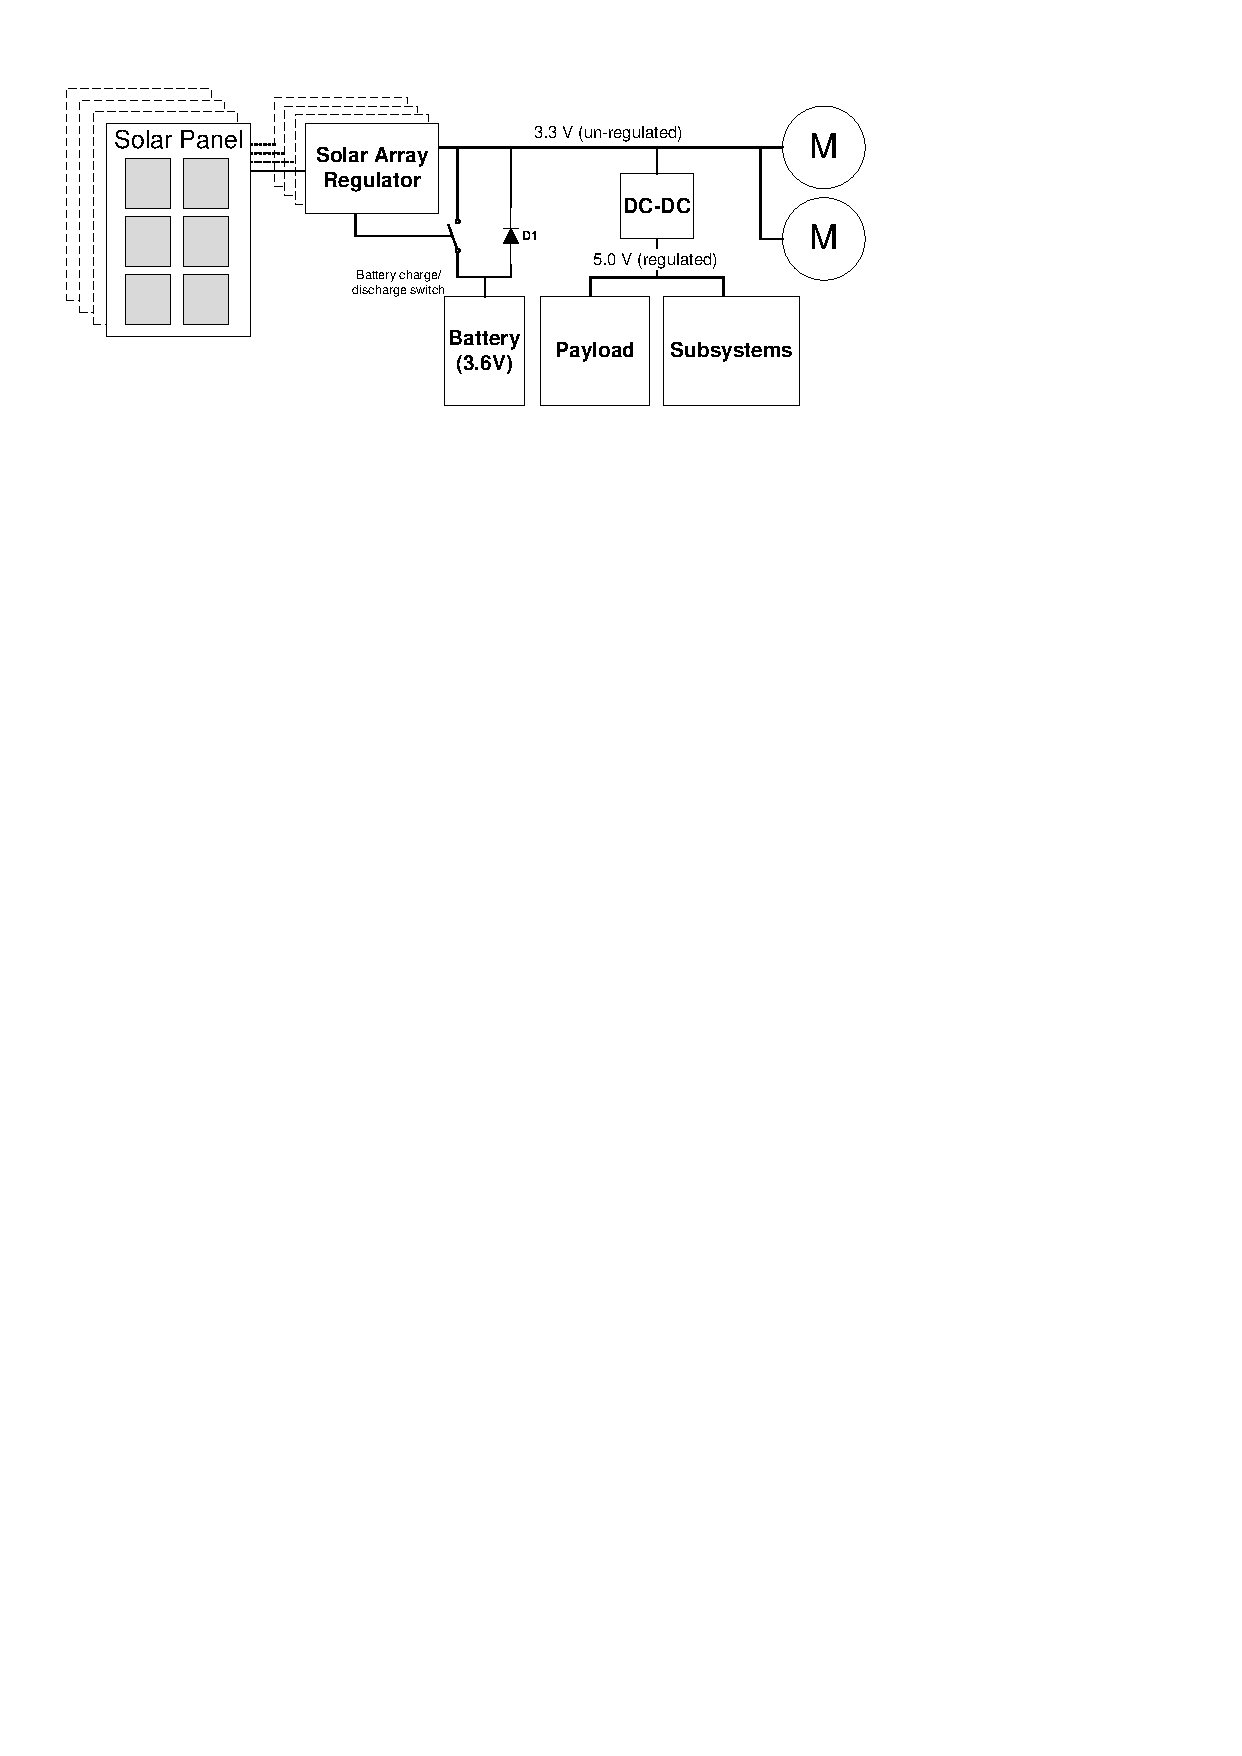
\includegraphics[scale=1]{figures/fig_PDR_EPSdiagram}
\caption{\ac{EPS} system diagram}
\label{fig:EPSdiagram}
\end{figure}
%
%
\subsection{Feasibility Study and Risk Analysis}
%How feasible is it to successfully implement the chosen concept? – Which potential issues/challenges might occur?
%
\subsubsection*{MPPT Regulator}
The \ac{MPPT} regulator is a relative large and complicated circuit requiring significant amount of man-hours to design, build and test. The responsible team has previous practical experience with both \acp{SAR} and \acp{MPPT} which is believed to drastically reduce the implementation time. With the \ac{MPPT} regulator, it is proposed first to build the DC-DC converter with output voltage control(feedback) thus resembling the shunt-regulator in functionality only with a few percent higher losses due to the DC-DC converter. This design allows one regulator to operate all four solar panels, since the \ac{MPPT} circuit is not yet included. Using this approach, it will be faster to build a first-prototype regulator, working as a backup plan, should the full \ac{MPPT} regulator prove to complicated to implement within the given project constraints. As a third backup, the extremely simple, but crude Zener-diode regulator can be implemented within very shot time, to provide a minimum amount of power.
%
\subsubsection*{Li-ion Battery}
Li-ion battery technology is widely spread used technology for modern computers and electronics. However, the technology requires more sophisticated protection circuitry against over-charge/discharge conditions, which can lead to a major system failure and potentially pose a safety risk. Extensive testing and use of application procedures should be applied.
%
\subsubsection*{Solar Arrays}
The solar arrays are the major contribution to the \ac{EPS} cost and mass budget. The proposed solar cells, \cite{MC_Solar_Cell}, list very promising specifications, however the credibility remains to be verified. If cheap and light-weight solar cells are not available, it will be a critical roadblock for realizing the project.
%
%
\subsection{Telemetry and Telecommands}
%What telemetries/telecommands are required/useful for the subsystem? – What data rates/sizes are required?
%
The required/recommended telemetry and telecommands, \ac{EPS} , are listed in table \ref{tab:Telemetry_Telecommands}.
%
\begin{table}[H]
\centering
\caption{Telemetry and telecommands}
\label{tab:Telemetry_Telecommands}
\begin{tabular}{|l|l|l|}
\hline
\textbf{Telemetry} & \textbf{Data rate/frequency} & \textbf{Data size} \\
\hline
Battery voltage & Every 30 sec & 1 byte \\
\hline
Solar array temperature & Every 30 sec & 1 byte\\
\hline
Solar array voltage & Every 1 sec(MPPT performance) & 2 bytes\\
\hline
Solar array current & Every 1 sec(MPPT performance) & 2 bytes\\
\hline%\hline
%\textbf{Telecommands} & \textbf{Parameters} & \textbf{Valid input range}\\
%set-output-voltage & $<voltage>[1 byte]$ & $0;255 (=???\,V$)\\
%\hline
\end{tabular}
\end{table}
%
\subsection{External Interfaces}
%How are the external interfaces implemented for the mechanics, power, communication etc.?
%
The interfaces of the \ac{EPS} external are listed in table \ref{tab:external_interfaces}.
%
\begin{table}[H]
\centering
\caption{External interfaces}
\label{tab:external_interfaces}
\begin{tabular}{m{0.35\textwidth}m{0.55\textwidth}}
\hline
\textbf{External interface} & \textbf{Implementation}\\
\hline
Solar array mounting to rigid ballon structure & Screws and bolts\\[2mm]
DC-DC regulators & Mounted on PCB which sits in system housing. Thermal contact points should be included, to remove internal heat dissipation.\\[2mm]
Voltage/current sensor telemetry & Analog signals to Microcontroller\\[2mm]
%Output voltage control(reference voltage setpoint) & Analog signal from Microcontroller\\[2mm]
Payload supply voltages & $3.3\,V$(unregulated) and $5.0\,V$(regulated)\\[2mm]
\hline
\end{tabular}
\end{table}
\section{Test and Verification of Design}
\label{sec:test_verification}
This section describes the various design models used to develop the \ac{EPS} along with the expected functional test to be executed.
%
\subsection{EPS Design Models}
%
\subsubsection{EPS PSpice Simulations}
A transient PSpice simulation model of the whole \ac{EPS} is currently being implemented. The completed PSpice models are shown in Appendix \ref{app:EPS_PSpice}. These will help in the design and testing of the regulator performance and system stability during transient loading as well as the interactions between the different circuits.

In future, it is desired also to implement transient PSpice models for the solar array\cite{Castaner}, \ac{MPPTU}, battery\cite{gold}, motors and \ac{BCR}.
%
\subsubsection{EPS Development Model}
An \ac{EPS} \ac{DM} is currently being build as seen in Figure \ref{fig:EPSprototype}. The prototype \ac{PCB} is realized using self-made "mini-mount" \ac{PCB} pads as shown in Appendix \ref{app:EPS_mini-mount}. These pads are attached, using a simple glue roller, on a complete copper ground plane. This design approach allows a compact layout which reduces parasitic effects. Also any \ac{IC} package can be supported and parts can easily be moved around if the design changes.
%
\begin{figure}[H]
\centering
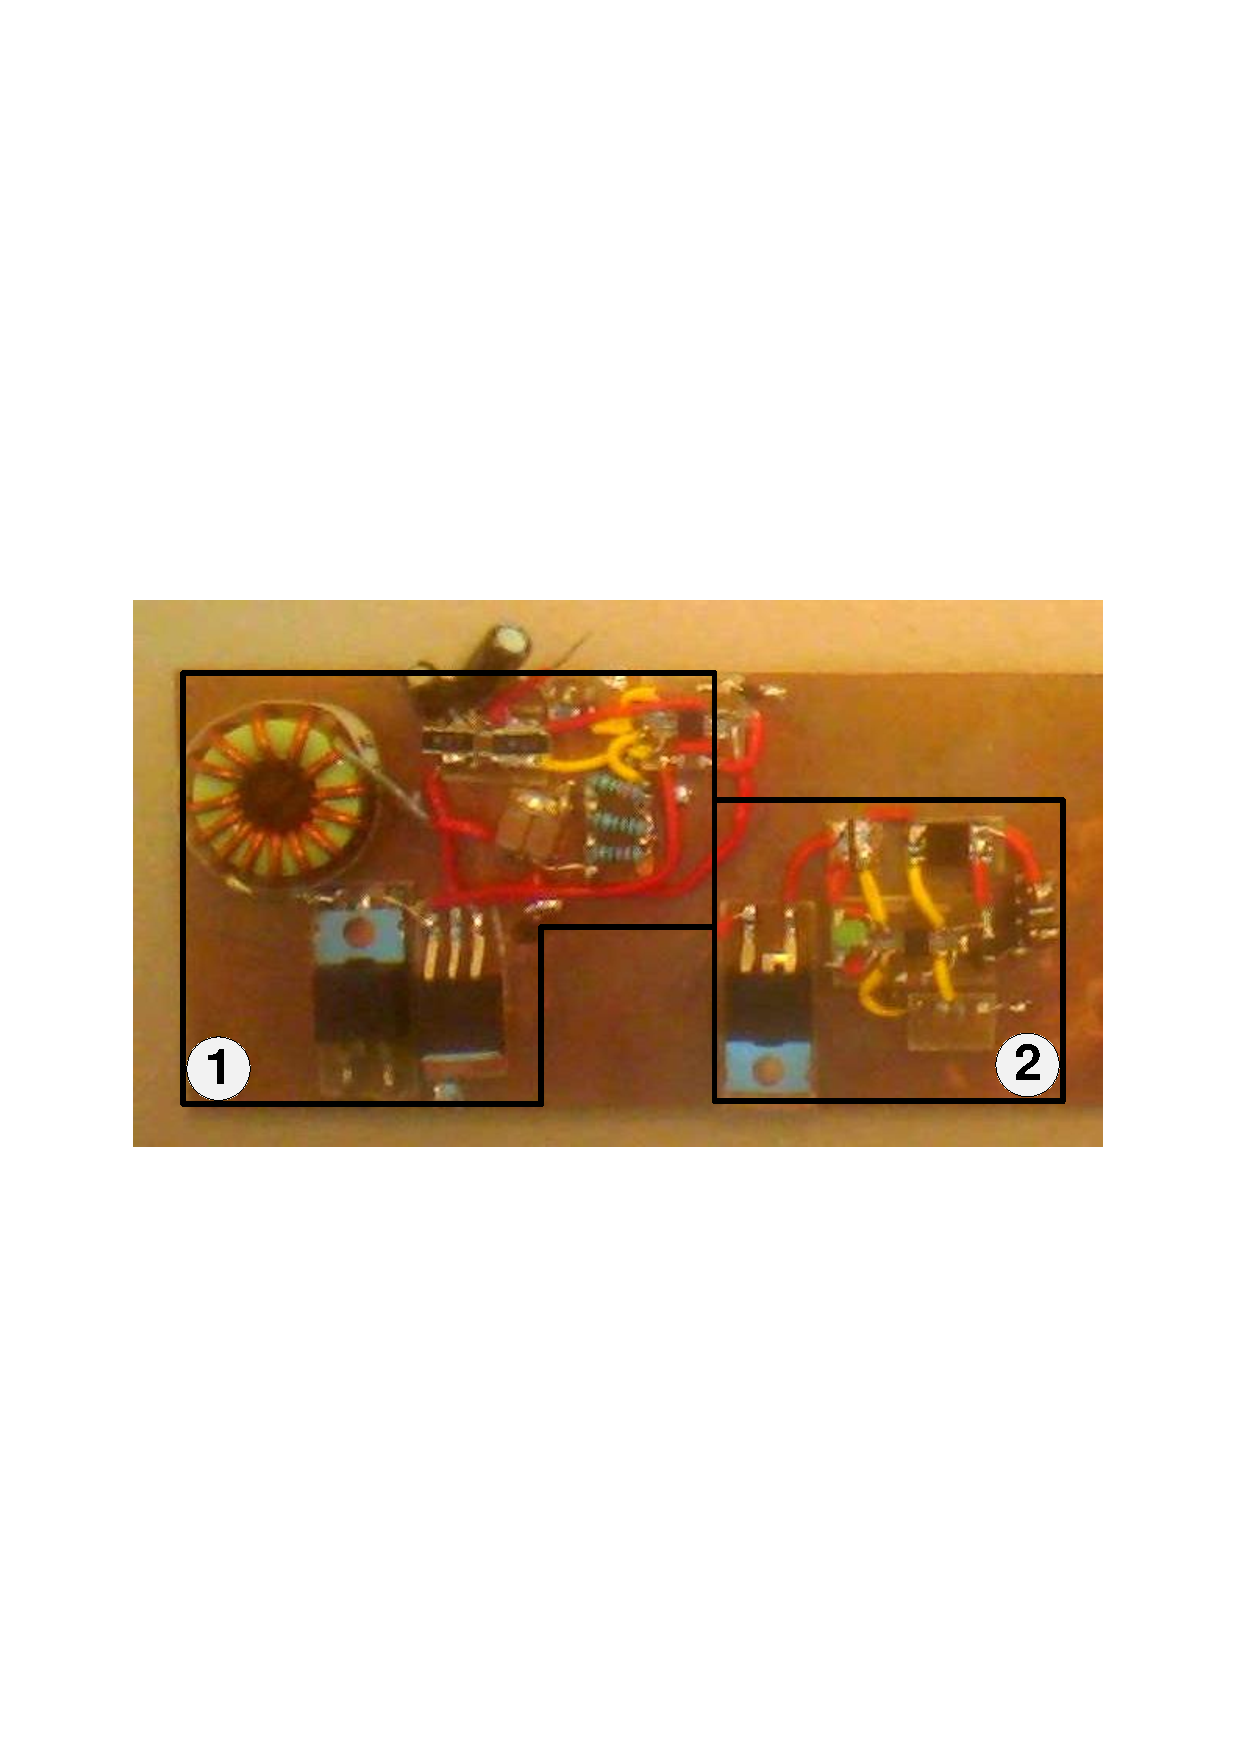
\includegraphics[width=0.8\textwidth]{figures/fig_CDR_EPSprototype}
\caption{\ac{EPS} prototype - \textbf{1}:\ac{SAR}, \textbf{2}:\ac{BCR}}
\label{fig:EPSprototype}
\end{figure}
%
\subsubsection*{Development Model Status}
The \ac{SAR} is working but shows signs of \ac{CM} instability which is expected to be caused by the missing current sense amplifier circuit and input filter. Development progress is currently awaiting delivery of components.

The \ac{BCR} is also working however excessive heating of the MOSFET was experienced. A new part rated for higher power dissipation has been selected and is currently awaiting delivery.
%
\subsubsection{EPS Flight Model}
If time allows, a dedicated \ac{FM} will be build, using a custom designed \ac{PCB} schematic layout. An optimized \ac{PCB} layout will minimize the system mass and size while maximizing the efficiency and system robustness.
%
\subsection{EPS Test Program}
Table \ref{tab:test_program} lists all necessary and desired test of the EPS. Priority "1" tests are all required while priority "2" tests will only be realized if time and resources allow it.
%
\begin{center}
\begin{longtable}[H]{p{0.15\textwidth}p{0.3\textwidth}p{0.45\textwidth}r}
\caption{EPS Test Program}\\
\label{tab:test_program}\\[-0.5cm]
\hline
\textbf{Subsystem} & \textbf{Condition/Mode} & \textbf{Test Description} & \textbf{Pri.}\\
\hline
\ac{SAR} & Mainbus voltage limitation & With more input power than load power, \ac{SAR} must be able to maintain a stable $9.5\,V$ output voltage also during transient loading & 1\\
- & Maximum power handling & With an input and load power slightly above the maximum expected solar array power, no \ac{SAR} components must overheat or otherwise malfunction & 1 \\
- & \ac{MPPT} & \ac{TBD} & 2\\
- & Mode transitions & \ac{SAR} must be able to change between \ac{MPPT}, battery charge and discharge mode without loosing mainbus voltage regulation or causing other malfunctions & 2\\
- & Feedback loop stability & Regulator bandwidth, gain- and phase margins should be measured with a Network Analyzer & 2\\
- & \ac{EMC} & Electromagnetic emissions should be measured with a Spectrum Analyzer, especially with concerns to the telecommunication systems & 2\\
\hline
\ac{BCR} & \ac{CC} and trickle charging & \ac{CC} charge at $2.4\,A$ and trickle charge mode entered when battery voltage reaches $8.4\,V$ should be verified & 1\\
- & Charge inhibit at high/low temperatures & While battery is charging, battery thermistor is heated/cooled in thermal oven/fridge to slightly above/below the specified temperature limits and charging should be terminated & 1\\
\hline
\ac{UVLO} & Power cut-off and recovery & Reducing input voltage below calculated threshold voltage should open switch and switch should close again when input voltage is increased above the threshold & 1\\
\hline
Battery & Dynamic model & Test approach is described in \cite{chen} & 2\\
\hline
Solar cell & I-V specifications & short-circuit current, open-circuit voltage, current and voltage at the \ac{MPP} should be determined from an irradiance test & 2\\
- & Temperature coefficients & Solar cell temperature coefficients should be determined be measuring the I-V characteristics at different temperatures within the expected temperature interval & 2\\
\hline
Fuses & Temperature variation & The \ac{PTC} resettable fuses should be tested at nominal, minimum and maximum expected temperatures to verify acceptable functionality & 1\\
\hline
\end{longtable}
\end{center}
%
\section{Resources and Scheduling}
\label{sec:resources_scheduling}

\subsection{Main Tasks}
some text...

\subsection{Parts List and Costs}
some text...

\subsection{Electronics Ground Support Equipment (EGSE)}
some text...

\subsection{Mechanical Ground Support Equipment (MGSE)}
some text...

\newpage
\printbibliography
\markboth{Bibliography}{Bibliography}
\addcontentsline{toc}{section}{\protect\numberline{}References}
\newgeometry{margin=1.5cm}
\pagestyle{plain}

\appendix

\chapter{Some Appendix}\label{app:SomeAppendix}
some text...

\chapter{Another Appendix}\label{app:AnotherAppendix}
some text...

%\includepdf{figures/bagside}

\end{document}
